\chapter{Теория}\label{ch:ch1}

Теоретическая часть данной работы будет описывать ту предметную область с которой пришлось столкнуться в ходе выполнения практической части.

\section{Поведение робота} \label{sec:robot-behavior}

Прежде чем перейти к определению поведения будущего робота мы должны определить его главную задачу. А именно - поиск целевых объектов в замкнутом пространстве.

Для того чтобы выполнить данную задачу робот должен уметь объезжать то замкнутое пространство в котором он находится, распознавать объекты и уметь подъезжать к найденному целевому объекту. Здесь можно выделить две возможные стратегии, которые можно применять к данной задаче:

\begin{enumerate}
\item Сначала выполняется объезд всего доступного пространства, во время которого строится карта местности, а затем происходит выполнение на ней поиска целевых объектов;
\item Целевой объект ищется непосредственно во время объезда пространства. При этом объезд пространства происходит без составления карты.
\end{enumerate} 

К преимуществам первого подхода можно записать:
\begin{itemize}
\item Помимо поиска целевых объектов выполняется полное сканирование местности, что может пригодится для других задач;
\item Возможно более <<умное>> построение маршрута при помощи, например, таких алгоритмов как A*\footnote{A* - алгоритм поиска по первому наилучшему совпадению на графе\cite[с. 218]{лорьер}.};
\item Можно найти все целевые объекты в данном замкнутом пространстве и примерно оценить их местоположение на отсканированной карте местности.
\end{itemize}

К недостаткам первого подхода относятся:
\begin{itemize}
\item Долгое время работы алгоритма: сначала нужно все объездить, оценить обстановку, а затем искать объекты;
\item Требуется более сложная алгоритмическая составляющая: как минимум роботу нужно научиться прокладывать маршруты на динамически строящейся карте и уметь определять себя и целевые объекты на ней\footnote{По сути требуется решить задачу SLAM};
\end{itemize}

У второго подхода есть хоть и одно, но очень большое преимущество и это относительно <<лёгкая>> реализация: как в алгоритмическом, так и в плане производительности. Не требуется составлять карт, а значит и решать задачу SLAM\footnote{SLAM - метод для построения или обновления карты в пространстве с одновременным контролем местоположения и пройденного пути\cite[с. 9]{aycock2010simultaneous}.}, в связи с этим уменьшается вычислительная нагрузка на робота.

Недостатки второго подхода:
\begin{itemize}
\item Время поиска целевого объекта будет зависеть от удачи, так как карты местности не строится и угадать когда робот поедет к целевому объекту не просто;
\item Полное сканирование местности не выполняется, а значит не все целевые объекты могут быть найдены в пространстве;
\end{itemize}

\section{Анализ окружающего пространства} \label{sec:environment-analysis}
%\fixme{Здесь пишем о том, какие виды анализа окружающего пространства могут быть задействованы, и какие полезные данные они могут привнести}

Основным сенсором при решении задачи визуального анализа окружающего пространства является видеокамера. Для того чтобы анализировать сигнал с видеокамеры требуется решить задачу машинного зрения. А именно требуется каким-то образом обрабатывать полученное изображение и исходя из этого строить стратегию движения.

Например, можно обучить нейронную сеть, которая распознаёт различные объекты и классифицирует их как опасные или целевые. Если робот видит опасный объект, он немедленно должен перестроить свой маршрут так, чтобы не столкнуться с ним. И если робот видит целевой объект, то он наооборот должен подъехать к нему, удостовериться в том, что это именно нужный целевой объект и сохранить его местоположение в энергонезависимой памяти.

В качестве дополнительного сенсора для визуального анализа пространства можно использовать также технологию Лидар, которая позволяет также получить некоторое изображение, представляющее собой облако точек, поддающееся анализу. По сути прибор, реализующий технологию Лидар представляет собой дальномер оптического диапазона, который замеряет угол и расстояние до точки (получаются полярные координаты) при помощи лазерного сканирования. Существует два основных типа сканирующих лидаров \cite[с. 702]{xiao2020proceedings}:

\begin{enumerate}
\item 3D лидар;
\item 2D лидар.
\end{enumerate} 

Первый позволяет получить 3D картинку. Обычно такой лидар оснащён подвижным лазером, который довольно долго сканирует перед собой окружающую местность. Однако, уже сейчас можно найти 3D лидары, которые сканируют с довольно быстрой скоростью\cite[с. 308]{hutter2017field}. Примером результата такой работы может стать картинка, изображённая на Рисунке~\ref{fig:3D-lidar-example}. На сегодняшний день такие лидары являются довольно дорогими устройствами.

%https://news.panasonic.com/global/presskits/ceatec2017
\begin{figure}[ht]
  \centerfloat{
    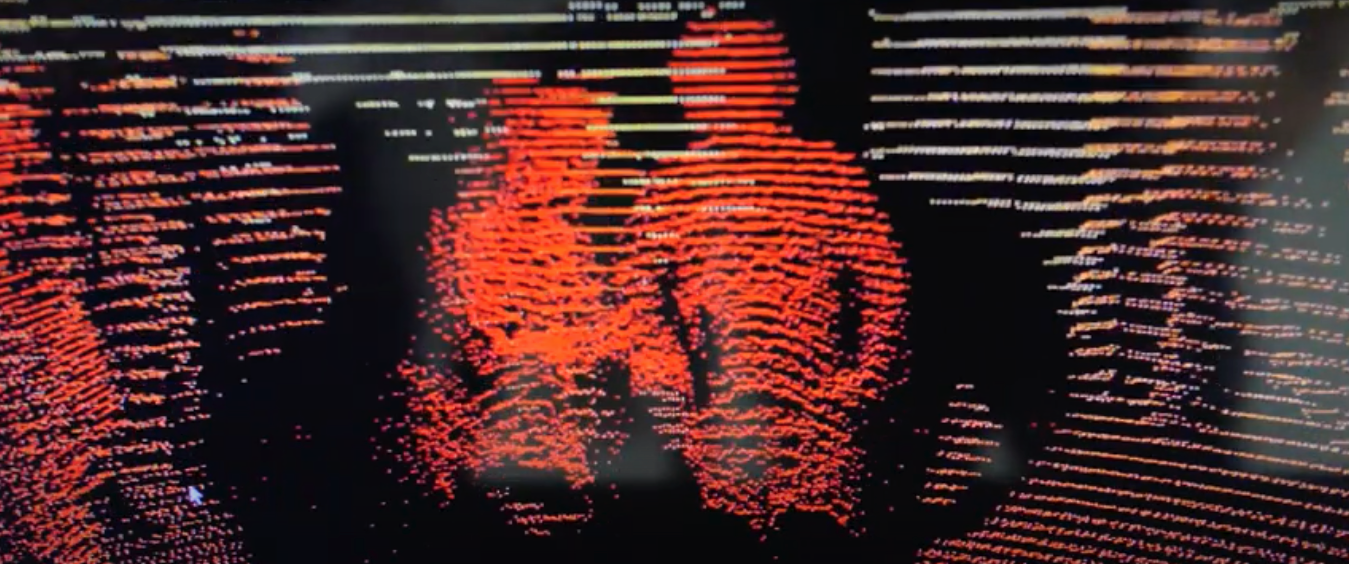
\includegraphics[scale=0.27]{3D-Lidar-Example.png}
  }
  \caption{Пример картинки, генерируемой 3D лидаром, представленном на выставке CEATEC 2017 компанией Panasonic в Японии.}\label{fig:3D-lidar-example}
\end{figure}

Второй соответственно уже создаёт двухмерное облако точек, которое также можно визуализировать в виде картинки, пример которой изображён на Рисунке \ref{fig:ydlidar-pointcloud}. Такой лидар обычно сканирует область вокруг себя и имеет угол обзора 360 градусов. Лазер также является подвижным, но только в этот раз он просто движется вокруг своей оси\cite[с. 610]{jia2019proceedings}.

\begin{figure}[ht]
  \centerfloat{
    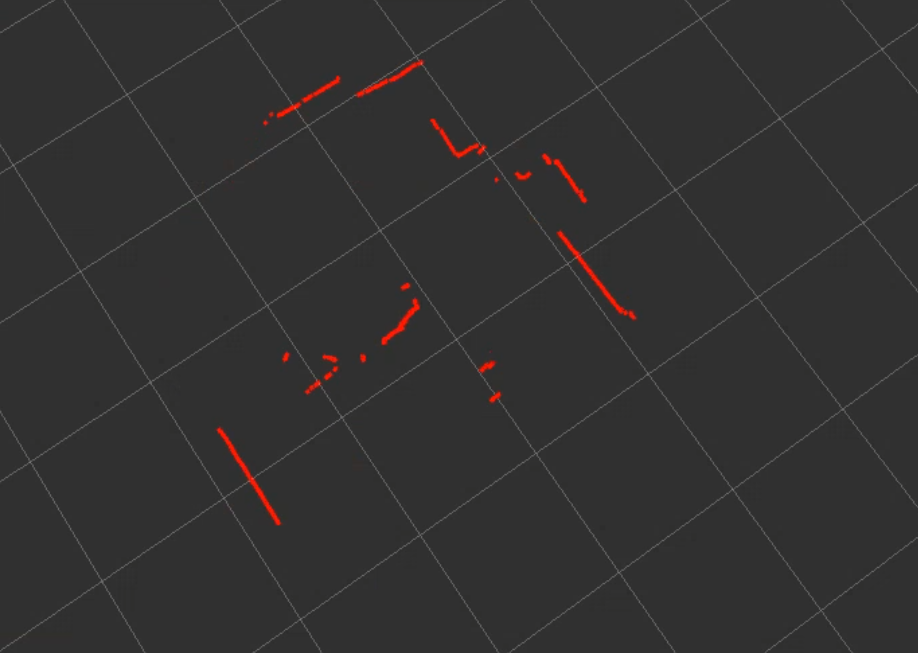
\includegraphics[scale=0.4]{ydlidar-pointcloud.png}
  }
  \caption{Пример картинки, генерируемой 2D лидаром YDLIDAR X4.}\label{fig:ydlidar-pointcloud}
\end{figure}

\section{Об управлении} \label{sec:about-driving}
%\fixme{Здесь пишем о том, какого виды хода бывают роботы и как они управляются}
Одна из задач, которую должен уметь решать мобильный автономный робот это задача передвижения. Потому как без него робот уже не будет полностью соответствовать своему критерию <<мобильности>>. Движение для робота, применительно к конкретной задаче данной ВКР просто необходимо. 

Для того чтобы робот двигался ему необходимо шасси. Шасси в основной своей массе по своей подвижной части подразделяются на те, что осуществляют езду при помощи гусеничной ленты и те, что ездят на колёсах. Шасси на гусеницах обладают большей проходимостью и мобильностью в следствии того, что гусеницы позволяют, например, разворачивать робота на месте.

Для того чтобы управлять шасси роботу необходимы электродвигатели и контроллер движения для них, но подробнее речь об этом зайдёт в пункте~\ref{sub:robot-move}. 

\FloatBarrier
